% Provenance (never printed): no school programme; the data strand of
% ../economics_series.md and the chart-reading notions of the principles textbooks.
% Mathematics owns percentages and chart reading (one-math-book g6
% proportionality-and-data); this chapter adds totals and per-person values, shares,
% rates of change and the times-ten scale. Brief: sources/book1/BRIEFS.md, g6-01.
\chapter{Reading Economic Charts}\label{ch:g6:reading-economic-charts}

Two hundred years ago, about one billion people lived on Earth. In 2022 there
were almost eight billion. Most of them live longer, eat better and earn more than
their great-great-grandparents did --- but not all of them, and not by the same
amount. How do we know? Nobody can see the whole world at once. What we can see
are numbers, collected by thousands of people over many years, and drawn as
charts.

This book opens with twenty-one of these charts. They show how people have
lived for two centuries: what they earned, how long they lived, where they
worked, what they ate and how they traded. Before looking at them, we learn to
read them. A chart is a tool, like a map: it is very useful to someone who
knows how to read it, and it can mislead someone who does not.

\begin{omfigure}
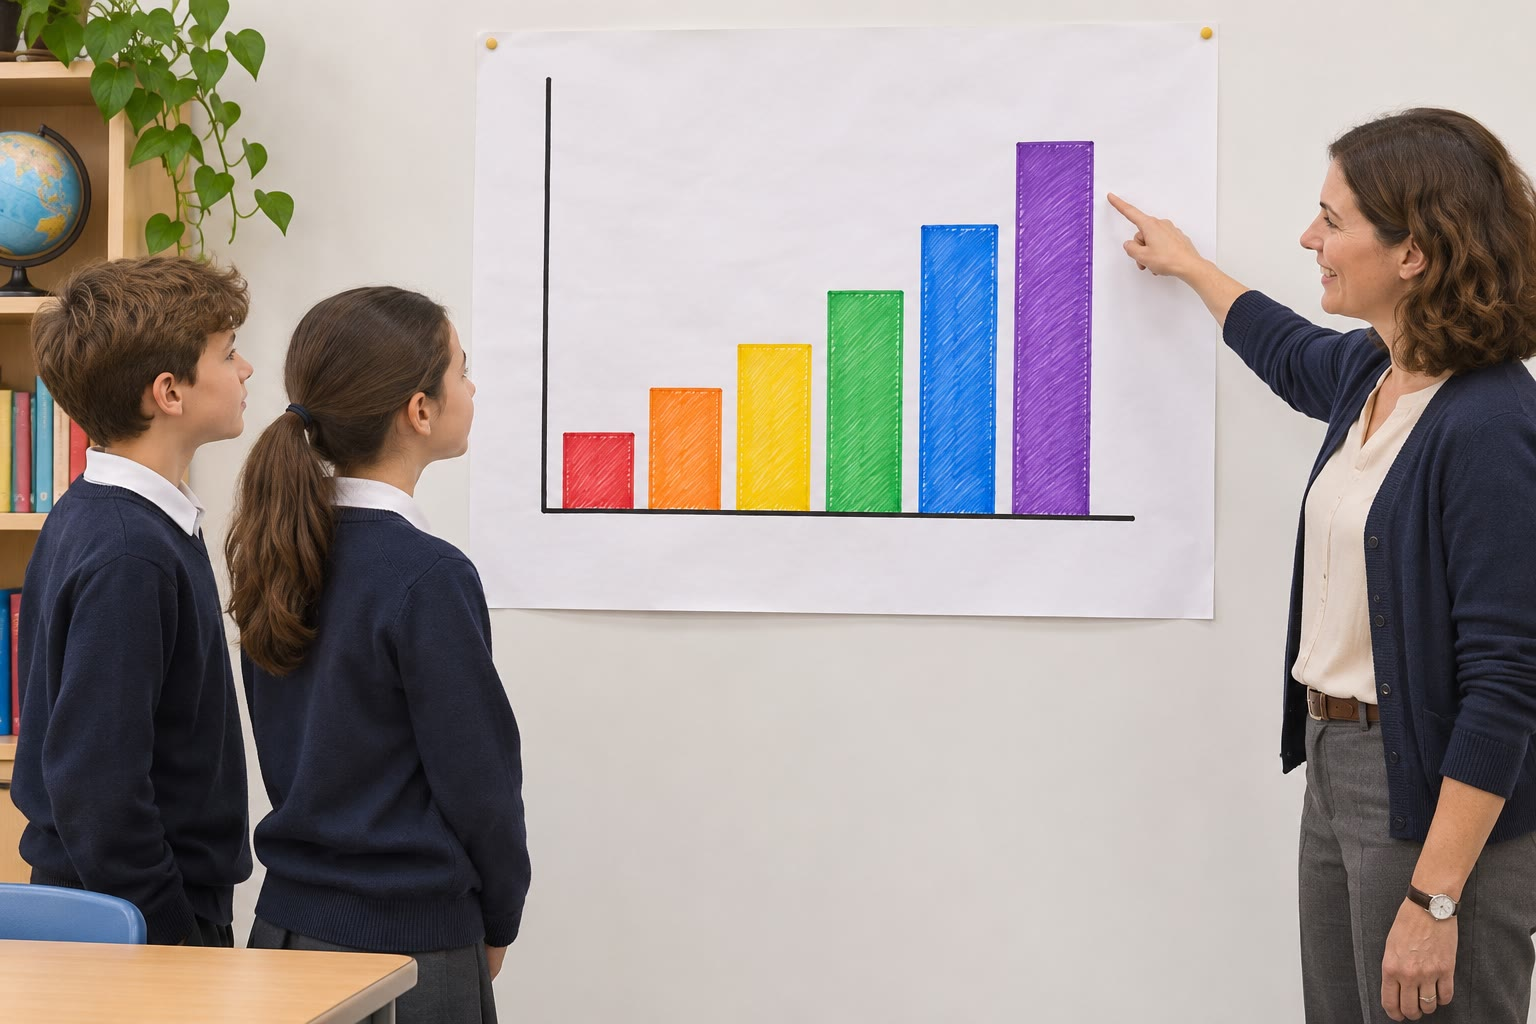
\includegraphics[width=0.62\linewidth]{images/book1/ai/g6-reading-economic-charts-classroom.jpg}

{\small A bar chart drawn by hand. Before believing a chart, a careful reader
asks what it measures, in what unit, and where its numbers come from.}
\end{omfigure}

\begin{recall}
A percentage is a number of parts out of 100: $25\,\%$ of a quantity is
$\frac{25}{100}$ of it. A line chart joins points placed against two axes; a
bar chart draws one bar per category, and the height of the bar is the value.
(The mathematics books show how to read and draw them.)
\end{recall}

\section{A quantity followed over time}

Economics is full of quantities that change from year to year: the number of
people in a country, the price of bread, the money a family earns. To see how
such a quantity changes, we write down its value year after year.

\begin{definition}[Time series]\label{def:g6:reading-economic-charts:time-series}
A \emph{time series}\index{time series} is a list of the values of one
quantity, measured in the same way at successive dates, written in the order
of the dates.
\end{definition}

A \omterm{def:g6:reading-economic-charts:time-series}{time series} is usually drawn as a line chart. The dates go along the
horizontal axis, from left to right; the values go up the vertical axis. Each
value is a point, and the points are joined by a line.

\begin{omchart}{World population, 1820--2022, in billions of people. Each dot
is one of the years for which the source gives a world estimate.}{Maddison Project Database 2023, regional data: population}
\begin{tikzpicture}
\begin{axis}[omtime, xlabel={Year}, ylabel={Billions of people},
  xmin=1810, xmax=2030, ymin=0, ymax=9, ytick={0,1,...,9}]
\addplot+[mark=*, mark size=1.3pt] table[x=year, y=pop_bn]
  {figdata/grade-6/01-reading-economic-charts/out/world_population.csv};
\end{axis}
\end{tikzpicture}
\end{omchart}

% figdata: world_population (1820 1.042; 1900 1.547; 1950 2.518; 2000 6.048; 2022 7.802)
The chart says that the world had about 1.0 billion people in 1820, about
1.5 billion in 1900, 2.5 billion in 1950, 6.0 billion in 2000 and 7.8 billion
in 2022. The line climbs slowly at first, then much faster after 1950. Reading a
chart means turning its shapes back into numbers like these.

\begin{method}[Reading a value off a line chart]\label{met:g6:reading-economic-charts:read-value}
To read the value of a quantity at a given date:
\begin{enumerate}
  \item find the date on the horizontal axis and go straight up to the line;
  \item from that point, go straight across to the vertical axis;
  \item read the value between the two nearest gridlines, and give it
        \emph{with its unit} (here: billions of people);
  \item round it: a value read off a chart is never exact. Give only as many
        digits as you can really see.
\end{enumerate}
\end{method}

\begin{example}[The world in 1900]\label{ex:g6:reading-economic-charts:1900}
Go up from 1900 to the line: the dot sits halfway between the gridlines 1 and
2. The world had about $1.5$ billion people in 1900. Saying ``$1.547$ billion''
would claim more than the chart shows; the number $1.547$ is in the table that
the chart was drawn from, not on the chart.
\end{example}

Under every chart of this book there is a line that starts with
\emph{Source}. It is as important as the chart itself.

\begin{definition}[Source line]\label{def:g6:reading-economic-charts:source-line}
The \emph{source line}\index{source line} of a chart names where its numbers
come from: the organisation or the researchers who collected them, and the
dataset they published. It lets any reader check the numbers, and judge how
far to trust them.
\end{definition}

\begin{measure}[Counting people]
Most countries now count their people in a \emph{census}: every household
fills in a form, once every five or ten years. Between two censuses, the
statistical office adds the births and the people who arrive, and takes away
the deaths and the people who leave. Two hundred years ago, very few countries
held a census. The number for 1820 in the chart above is therefore an
\emph{estimate}: researchers built it from tax lists, church registers of
baptisms and burials, and counts of villages and towns. It could be wrong by
a tenth or more. The \omterm{def:g6:reading-economic-charts:source-line}{source line} tells us who made the estimate --- here, the
team that publishes the Maddison Project Database --- so that we can read how
they made it.
\end{measure}

The parts of a chart are always the same, whatever it shows.

\begin{omfigure}
\begin{tikzpicture}[econ, x=1cm, y=1cm]
  % frame of a model chart (an invented line: this is a diagram, not data)
  \draw[black!80] (0,0) -- (6,0);
  \draw[black!80] (0,0) -- (0,3.6);
  \foreach \y/\l in {0/0, 1.2/100, 2.4/200, 3.6/300} {
    \draw[gray!30] (0,\y) -- (6,\y);
    \node[left, font=\scriptsize] at (0,\y) {\l};
  }
  \foreach \x/\l in {0/2000, 2/2010, 4/2020, 6/2030} {
    \node[below, font=\scriptsize] at (\x,0) {\l};
  }
  \draw[omDef, thick] (0,0.9) -- (1,1.1) -- (2,1.0) -- (3,1.6) -- (4,2.1) -- (5,2.0) -- (6,2.7);
  \draw[omThm, thick] (0,0.5) -- (1,0.6) -- (2,0.8) -- (3,0.8) -- (4,1.0) -- (5,1.3) -- (6,1.4);
  \node[font=\scriptsize, fill=white, inner sep=1pt, anchor=west] at (0.2,3.25) {\textcolor{omDef}{---} Town A\quad\textcolor{omThm}{---} Town B};
  \node[font=\scriptsize\itshape, anchor=north west, text=black!70] at (-0.6,-0.6) {Source: Brenmoor town hall, invented data};
  \node[font=\scriptsize, rotate=90] at (-1.0,1.8) {Thousands of loaves};
  \node[font=\small\bfseries] at (3,4.3) {Loaves bought in two towns};
  % labels of the parts
  \begin{scope}[every node/.style={font=\footnotesize, align=left, anchor=west, text=omExo!80!black}]
    \node (t) at (7.0,4.3) {title: what is shown};
    \node (l) at (7.0,3.0) {legend: which line is which};
    \node (g) at (7.0,3.65) {gridlines, to read values};
    \node (h) at (7.0,0.3) {horizontal axis: the dates};
    \node (s) at (7.0,-0.75) {source line};
    \node[anchor=east] (u) at (-1.3,4.3) {unit of the\\vertical axis};
  \end{scope}
  \begin{scope}[omExo!80!black, ->, thin]
    \draw (t.west) -- (5.6,4.3);
    \draw (l.west) -- (3.45,3.2);
    \draw (g.west) -- (6.08,3.6);
    \draw (h.west) -- (6.08,0.03);
    \draw (s.west) -- (5.45,-0.75);
    \draw (u.south) -- (-1.0,3.15);
  \end{scope}
\end{tikzpicture}

{\small The parts of a chart, on an invented example: two towns and the
number of loaves of bread they buy each year.}
\end{omfigure}

\section{Totals, per person, and shares}

A big country produces more food than a small one, and pays more taxes, and
buys more bicycles, simply because it has more people. To compare countries
of different sizes, economists divide by the number of people.

\begin{definition}[Total and per-person values]\label{def:g6:reading-economic-charts:per-person}
The \emph{total value}\index{total value} of a quantity is its amount for a
whole group: a town, a country, the world. Its \emph{per-person
value}\index{per-person value} is the total divided by the number of people
in the group:
\[
  \text{per-person value} = \frac{\text{total value}}{\text{number of people}}.
\]
A per-person value is also called a value \emph{per capita} (Latin for ``per
head'').
\end{definition}

\begin{example}[Rice in two villages]\label{ex:g6:reading-economic-charts:rice}
In a year, a village of 2\,000 people harvests 500\,000 kilograms of rice,
and a village of 500 people harvests 200\,000 kilograms (invented numbers).
The first village has the larger total. Per person, it harvests
$500\,000 \div 2\,000 = 250$ kilograms, and the second village
$200\,000 \div 500 = 400$ kilograms. The small village has the larger
per-person harvest.
\end{example}

A \omterm{def:g6:reading-economic-charts:per-person}{per-person value} is an \emph{average}: it says how much each person would
have if the total were shared out equally. It never says that the total
\emph{is} shared out equally. Two villages with the same rice per person can
be very different: in one, every family has about the same; in the other, a
few families own most of the harvest.

Often we want to know not how much of something there is, but how big a part
of a whole it is.

\begin{definition}[Share of a total]\label{def:g6:reading-economic-charts:share}
The \emph{share}\index{share (of a total)} of a part in a total is the part
divided by the total, written as a percentage:
\[
  \text{share} = \frac{\text{part}}{\text{total}} \times 100\,\%.
\]
When a total is cut into parts that do not overlap, the shares of all the
parts add up to $100\,\%$.
\end{definition}

The next chart cuts the world's population into the eight large regions used
by the source, for five years. Each bar is the whole world, $100\,\%$; each
coloured piece is the \omterm{def:g6:reading-economic-charts:share}{share} of one region.

\begin{omchart}{Where the world's people live: the share of each region in
world population, in percent, for five years.}{Maddison Project Database 2023, regional data: population. ``Western
Offshoots'' are the United States, Canada, Australia and New Zealand}
\begin{tikzpicture}
\begin{axis}[omrecord, ybar stacked, bar width=15pt, width=0.8\linewidth,
  height=0.62\linewidth, ymin=0, ymax=100, ylabel={Percent of world population},
  symbolic x coords={1820,1870,1950,1990,2022}, xtick=data, grid=none,
  ytick={0,20,...,100}, ymajorgrids,
  legend style={at={(0.5,-0.12)}, anchor=north, legend columns=2},
  cycle list={{fill=omDef!80, draw=white}, {fill=omDef!35, draw=white},
    {fill=omProp!70, draw=white}, {fill=omThm!75, draw=white},
    {fill=omMeth!75, draw=white}, {fill=omMeth!35, draw=white},
    {fill=omDebate!55, draw=white}, {fill=black!30, draw=white}}]
\pgfplotsforeachungrouped \col in {east_asia, south_se_asia, mena, ssa,
    western_europe, eastern_europe, western_offshoots, latin_america} {
  \addplot+[] table[x=year, y=\col]
    {figdata/grade-6/01-reading-economic-charts/out/population_shares.csv};
}
\legend{East Asia, South and South-East Asia, Middle East and North Africa,
  Sub-Saharan Africa, Western Europe, Eastern Europe, Western Offshoots,
  Latin America}
\end{axis}
\end{tikzpicture}
\end{omchart}

% figdata: population_shares (east_asia 1820 41.1, 2022 21.0; ssa 1820 5.8, 1950 7.1, 2022 15.1;
% western_europe 1820 13.4, 2022 5.5; south_se_asia 2022 32.6)
In 1820, East Asia --- above all China --- held $41.1\,\%$ of the world's
people: two people in every five. In 2022 its \omterm{def:g6:reading-economic-charts:share}{share} was $21.0\,\%$. The \omterm{def:g6:reading-economic-charts:share}{share} of
Sub-Saharan Africa went the other way: $5.8\,\%$ in 1820, $7.1\,\%$ in 1950,
$15.1\,\%$ in 2022. Western Europe's \omterm{def:g6:reading-economic-charts:share}{share} fell from $13.4\,\%$ to $5.5\,\%$.

\begin{remark}[Percentage points]\label{rem:g6:reading-economic-charts:points}
When a \omterm{def:g6:reading-economic-charts:share}{share} goes from $41.1\,\%$ to $21.0\,\%$, it falls by
$41.1 - 21.0 = 20.1$ \emph{percentage points}. A difference between two
percentages is counted in percentage points, so that it cannot be confused
with a percentage \emph{of} something. \Cref{sec:g6:reading-economic-charts:rates}
explains the difference.
\end{remark}

A falling \omterm{def:g6:reading-economic-charts:share}{share} does not mean a falling number. A \omterm{def:g6:reading-economic-charts:share}{share} is a part of a total,
and the total here grew more than seven times.

\begin{example}[A smaller share of a bigger world]\label{ex:g6:reading-economic-charts:east-asia}
% figdata: world_population (1820 1.042, 2022 7.802); population_shares (east_asia 41.1, 21.0)
In 1820 the world had $1.042$ billion people, and East Asia's \omterm{def:g6:reading-economic-charts:share}{share} was
$41.1\,\%$, so East Asia had about
\[
  1.042 \times \frac{41.1}{100} \approx 0.43 \text{ billion people.}
\]
In 2022 the world had $7.802$ billion people and the \omterm{def:g6:reading-economic-charts:share}{share} was $21.0\,\%$:
$7.802 \times 0.210 \approx 1.64$ billion people. The \omterm{def:g6:reading-economic-charts:share}{share} of East Asia was
halved, while the number of its people was multiplied by almost four.
\end{example}

\section{Rates of change}\label{sec:g6:reading-economic-charts:rates}

The world had $2.518$ billion people in 1950 and $6.048$ billion in 2000.
% figdata: world_population (1950 2.518; 2000 6.048)
It gained $6.048 - 2.518 = 3.530$ billion people. Is that a lot? It depends on
where it started: $3.5$ billion more would be a huge change for a world of one
billion, and a small one for a world of a hundred billion. So we compare the
change with the starting value.

\begin{definition}[Rate of change]\label{def:g6:reading-economic-charts:rate-of-change}
The \emph{rate of change}\index{rate of change} of a quantity between two
dates is its change divided by its value at the first date, written as a
percentage:
\[
  \text{rate of change}
  = \frac{\text{later value} - \text{earlier value}}{\text{earlier value}}
    \times 100\,\%.
\]
When the later value is larger, the rate of change is a \emph{rise}; when it
is smaller, we compute $\frac{\text{earlier} - \text{later}}{\text{earlier}}
\times 100\,\%$ and call it a \emph{fall}.
\end{definition}

\begin{method}[Computing a rate of change]\label{met:g6:reading-economic-charts:rate}
\begin{enumerate}
  \item Write the earlier and the later values, in the same unit.
  \item Subtract the smaller from the larger: that is the size of the change.
  \item Divide by the \emph{earlier} value --- always the earlier one, never
        the later one.
  \item Multiply by 100, round, and say whether it is a rise or a fall.
\end{enumerate}
\end{method}

\begin{example}[World population, 1950 to 2000]\label{ex:g6:reading-economic-charts:pop-rise}
The change is $3.530$ billion, and $3.530 \div 2.518 \approx 1.40$. The world
population rose by about $140\,\%$ in fifty years. A rise of $100\,\%$ would
have doubled it; a rise of $140\,\%$ means that the 2000 population was
$2.4$ times the 1950 population.
\end{example}

\begin{example}[A fall: the United Kingdom in 2020]\label{ex:g6:reading-economic-charts:uk-fall}
% figdata: uk_income (2019 39113; 2020 34651)
Income per person in the United Kingdom was $39\,113$ dollars in 2019 and
$34\,651$ dollars in 2020, the year of the pandemic. The change is
$39\,113 - 34\,651 = 4\,462$ dollars, and $4\,462 \div 39\,113 \approx 0.114$:
a fall of about $11\,\%$ in one year. (The dollars are of a fixed value, as the
next chapter explains, so the fall is a real one, not a change in prices.)
\end{example}

\begin{remark}[Two traps]\label{rem:g6:reading-economic-charts:traps}
First, a rise and a fall of the same percentage do not cancel. A price that
rises by $50\,\%$, from 10 to 15, and then falls by $50\,\%$ ends at
$7.5$, because the second $50\,\%$ is taken of 15. Second, a fall can never be
more than $100\,\%$: a fall of $100\,\%$ already brings a quantity down to
zero. A rise has no such limit: from 1 to 10 is a rise of $900\,\%$.
\end{remark}

A \omterm{def:g6:reading-economic-charts:rate-of-change}{rate of change} over fifty years is not fifty times a rate over one year.
How a yearly rate builds up, year on year, is the subject of a later year of
this course. For now, rates of change compare two dates.

\section{The times-ten scale}

On the vertical axis of an ordinary chart, equal steps mean equal amounts:
from 0 to 1 billion is as far as from 6 to 7 billion. This becomes a problem
when a quantity grows very large. The next chart shows the income per person
of the United Kingdom since 1820, measured in dollars of fixed value (the next
chapter explains how). Look first at the left panel.

\begin{omchart}{Income per person in the United Kingdom, 1820--2022, in 2011
dollars of fixed purchasing power: the same numbers drawn on an ordinary scale
(left) and on a times-ten scale (right).}{Maddison Project Database 2023: GDP per person, United Kingdom}
\begin{tikzpicture}
\begin{groupplot}[group style={group size=2 by 1, horizontal sep=1.5cm},
  omtime, width=0.43\linewidth, height=0.4\linewidth, xmin=1820, xmax=2022,
  xtick={1850,1900,1950,2000}, xlabel={Year}]
\nextgroupplot[ymin=0, ymax=40000, ytick={0,10000,20000,30000,40000},
  ylabel={Dollars per person}, title={\small Ordinary scale}]
\addplot table[x=year, y=gdppc]
  {figdata/grade-6/01-reading-economic-charts/out/uk_income.csv};
\nextgroupplot[ymode=log, omtimesten, width=0.43\linewidth, height=0.4\linewidth,
  xmin=1820, xmax=2022, xtick={1850,1900,1950,2000}, ymin=1000, ymax=100000,
  minor ytick={2000,3000,4000,5000,6000,7000,8000,9000,20000,30000,40000,50000,60000,70000,80000,90000},
  yminorgrids, minor grid style={gray!12, line width=0.2pt},
  title={\small Times-ten scale}]
\addplot table[x=year, y=gdppc]
  {figdata/grade-6/01-reading-economic-charts/out/uk_income.csv};
\end{groupplot}
\end{tikzpicture}
\end{omchart}

% figdata: uk_income (1820 3306; 1900 7594; 1950 11061; 2000 31946; 2022 38406)
On the left, the line from 1820 to 1900 looks almost flat. Yet over those
eighty years income per person rose from $3\,306$ to $7\,594$ dollars: it was
multiplied by $2.3$. The ordinary scale squeezes it, because the axis must also
make room for the $38\,406$ dollars of 2022. On the right, the same eighty
years climb clearly. This is the second kind of scale.

\begin{definition}[Times-ten scale]\label{def:g6:reading-economic-charts:times-ten-scale}
On a \emph{times-ten scale}\index{times-ten scale}, the gridlines of the
vertical axis are placed at equal distances, and each gridline is ten times
the one below it: 1, 10, 100, 1\,000, 10\,000\ldots{} Two values that are
the same number of times larger than each other are always the same distance
apart.
\end{definition}

The small ticks between two gridlines mark 2, 3, 4\ldots\ 9 times the lower
gridline. They get closer and closer as they go up, because going from 1\,000
to 2\,000 doubles the value, while going from 9\,000 to 10\,000 adds only a
ninth.

\begin{omfigure}
\begin{tikzpicture}[econ, x=1cm, y=1cm]
  % left: ordinary ruler 0..10000; right: times-ten ruler 1..10000 (log10 positions)
  \draw[thick] (0,0) -- (0,6);
  \foreach \v/\l in {0/0, 2/2\,000, 4/4\,000, 6/6\,000, 8/8\,000, 10/10\,000} {
    \draw (-0.1,{\v*0.6}) -- (0.1,{\v*0.6});
    \node[left, font=\scriptsize] at (-0.1,{\v*0.6}) {\l};
  }
  \node[font=\footnotesize, align=center] at (0,-1.0) {ordinary scale:\\equal steps add\\the same amount};
  \draw[thick] (5,0) -- (5,6);
  \foreach \p/\l in {0/1, 1/10, 2/100, 3/1\,000, 4/10\,000} {
    \draw (4.9,{\p*1.5}) -- (5.1,{\p*1.5});
    \node[left, font=\scriptsize] at (4.9,{\p*1.5}) {\l};
  }
  \foreach \k in {2,...,9} {
    \draw (4.95,{(3+log10(\k))*1.5}) -- (5.05,{(3+log10(\k))*1.5});
  }
  \node[font=\footnotesize, align=center] at (5,-1.0) {times-ten scale:\\equal steps multiply\\by the same number};
  % the value 5000 on both rulers
  \fill[omThm] (0,3) circle (2pt);
  \node[right, font=\scriptsize, text=omThm] at (0.15,3) {5\,000};
  \fill[omThm] (5,{(3+log10(5))*1.5}) circle (2pt);
  \node[right, font=\scriptsize, text=omThm] at (5.15,{(3+log10(5))*1.5}) {5\,000};
  % equal steps on the times-ten ruler
  \draw[omDef, <->] (5.9,1.5) -- (5.9,3) node[midway, right, font=\scriptsize, align=left] {$\times 10$};
  \draw[omDef, <->] (5.9,3) -- (5.9,4.5) node[midway, right, font=\scriptsize, align=left] {$\times 10$};
  \draw[omDef, <->] (5.9,4.5) -- (5.9,6) node[midway, right, font=\scriptsize, align=left] {$\times 10$};
\end{tikzpicture}

{\small Two rulers from 0 (or 1) to 10\,000. On the ordinary scale, 5\,000
is halfway up. On the \omterm{def:g6:reading-economic-charts:times-ten-scale}{times-ten scale}, each step multiplies by ten, so
5\,000 sits high in the top step; the small ticks mark 2\,000, 3\,000,
\ldots, 9\,000.}
\end{omfigure}

\begin{method}[Reading a times-ten chart]\label{met:g6:reading-economic-charts:times-ten}
\begin{enumerate}
  \item Find the two gridlines between which the point lies: the value is
        between them (for example between 1\,000 and 10\,000).
  \item Use the small ticks to say ``about 3\,000'' or ``about 7\,000''.
  \item To compare two points, count the steps between them: one step is
        ten times, two steps a hundred times, half a step about three times.
  \item A straight line going up means that the quantity is multiplied by
        the same number in each equal stretch of time.
\end{enumerate}
\end{method}

\begin{example}[Reading the United Kingdom on both scales]\label{ex:g6:reading-economic-charts:uk-scales}
% figdata: uk_income (1820 3306; 1870 5829; 1920 7017; 1940 10928; 1970 17162; 2020 34651)
On the times-ten panel, the line starts at about 3\,000 dollars, between the
1\,000 and 10\,000 gridlines, crosses the 10\,000 gridline around 1940, and
ends just under 40\,000. On the ordinary panel, the line seems to shoot up
after 1950, as if something new had started. The times-ten panel corrects the
impression. Income per person was multiplied by $1.8$ from 1820 to 1870
($5\,829 \div 3\,306$), by $1.2$ from 1870 to 1920, by $2.4$ from 1920 to 1970
and by $2.0$ from 1970 to 2020. Growth was faster after 1920, but no
fifty-year stretch came near multiplying income by ten. The steepness of the
left panel comes mostly from the larger starting value: the same \omterm{def:g6:reading-economic-charts:rate-of-change}{rate of
change} adds many more dollars when the starting value is larger.
\end{example}

\begin{remark}[Which scale to use]\label{rem:g6:reading-economic-charts:which}
Use an ordinary scale to compare amounts: how many more dollars, how many more
people. Use a \omterm{def:g6:reading-economic-charts:times-ten-scale}{times-ten scale} to compare how many times larger, and to see
values that are very small and very large on the same chart. A \omterm{def:g6:reading-economic-charts:times-ten-scale}{times-ten scale}
has no 0: each step down divides by ten, and no number of steps reaches zero.
Always look at the vertical axis before reading the shape of a line.
\end{remark}

\section{What a chart cannot tell}

The charts of this chapter say that the world's population rose, that the
\omterm{def:g6:reading-economic-charts:share}{share} of some regions fell and others rose, and that income per person in the
United Kingdom rose more than ten times. They do not say \emph{why}. The
population chart does not tell whether people had more children, or whether
fewer children died; a later chapter shows that it was mostly the second. The
income chart does not tell whether the higher income came from new machines,
from more hours of work, from trade, or from something else; finding out is
the work of later years. A chart shows what happened. It does not show what
caused it.

Nor does an average tell how a total is shared. Income per person in the
United Kingdom in 2022 was $38\,406$ dollars, but no British family is
``the average family'', and many earned far less or far more.

\begin{method}[Five questions to ask any chart]\label{met:g6:reading-economic-charts:five}
\begin{enumerate}
  \item \textbf{What} quantity is shown, and is it a total, a \omterm{def:g6:reading-economic-charts:per-person}{per-person
        value}, a \omterm{def:g6:reading-economic-charts:share}{share} or a \omterm{def:g6:reading-economic-charts:rate-of-change}{rate of change}?
  \item In what \textbf{unit}, and over which dates or which places?
  \item On what \textbf{scale}: ordinary or times-ten? Does the vertical axis
        start at zero?
  \item What is the \textbf{source}, and how could the numbers have been
        collected?
  \item What does the chart \textbf{not} show: causes, differences hidden by
        an average, the years or places left out?
\end{enumerate}
\end{method}

The next six chapters use these five questions on eighteen more charts.

\section{Exercises}

\begin{exercise}[$\star$]\label{exo:g6:reading-economic-charts:1}
Use the chart of world population. (a) About how many people lived on Earth
in 1900, and in 2000? (b) By about how many billion people did the world grow
between these two dates?
\end{exercise}

\begin{exercise}[$\star$]\label{exo:g6:reading-economic-charts:2}
A village of 400 people harvests 120\,000 kilograms of potatoes in a year.
Another village of 1\,000 people harvests 200\,000 kilograms (invented
numbers). (a) Which village has the larger total harvest? (b) Compute the
harvest per person in each village. Which is larger?
\end{exercise}

\begin{exercise}[$\star$]\label{exo:g6:reading-economic-charts:3}
Use the chart of the regions' \omterm{def:g6:reading-economic-charts:share}{shares} of world population. (a) Which region had
the largest \omterm{def:g6:reading-economic-charts:share}{share} in 1820? Which had the largest \omterm{def:g6:reading-economic-charts:share}{share} in 2022? (b) Using the
values given in the text, by how many percentage points did the \omterm{def:g6:reading-economic-charts:share}{share} of
East Asia fall between 1820 and 2022?
\end{exercise}

\begin{exercise}[$\star$]\label{exo:g6:reading-economic-charts:4}
In a class of 25 pupils, 15 walk to school, 6 come by bus and 4 come by car.
(a) Compute the \omterm{def:g6:reading-economic-charts:share}{share} of each way of coming to school. (b) Check that the three
\omterm{def:g6:reading-economic-charts:share}{shares} add up to $100\,\%$.
\end{exercise}

\begin{exercise}[$\star\star$]\label{exo:g6:reading-economic-charts:5}
% figdata: uk_income (1950 11061; 2000 31946)
Income per person in the United Kingdom was $11\,061$ dollars in 1950 and
$31\,946$ dollars in 2000. (a) Compute the \omterm{def:g6:reading-economic-charts:rate-of-change}{rate of change} between the two dates.
(b) How many times larger was income per person in 2000 than in 1950?
\end{exercise}

\begin{exercise}[$\star\star$]\label{exo:g6:reading-economic-charts:6}
Use the times-ten panel of the chart of income per person in the United
Kingdom. Between which two gridlines does the line lie (a) in 1820, (b) in
1900, (c) in 2022? (d) About when does the line cross the 10\,000 gridline?
\end{exercise}

\begin{exercise}[$\star\star$]\label{exo:g6:reading-economic-charts:7}
A times-ten chart has gridlines at 10, 100, 1\,000, 10\,000 and 100\,000.
(a) A point moves up by two gridlines. How many times larger has the value
become? (b) How many gridlines separate 1\,000 and 100\,000? (c) A value is
multiplied by one thousand. By how many gridlines does its point move up?
\end{exercise}

\begin{exercise}[$\star\star$]\label{exo:g6:reading-economic-charts:8}
A newspaper prints the chart of world population and writes underneath:
``This chart proves that food became cheaper.'' (a) What does the chart show?
(b) Why does it not show what the newspaper says? (c) What chart would you
need to see in order to check the newspaper's claim?
\end{exercise}

\begin{exercise}[$\star\star$]\label{exo:g6:reading-economic-charts:9}
A bar chart compares income per person in two invented countries: Northland,
9\,500 dollars, and Southland, 10\,500 dollars. Its vertical axis starts at
9\,000, not at 0, and it has no \omterm{def:g6:reading-economic-charts:source-line}{source line}. (a) How tall is each bar above
the bottom of the axis, in dollars? How many times taller does Southland's bar
look? (b) How many times larger is Southland's income per person really? Round
to two decimals. (c) What should a careful reader ask about this chart?
\end{exercise}

\begin{exercise}[$\star\star\star$]\label{exo:g6:reading-economic-charts:10}
Two invented islands use the same money, the dalen. Island A has
2\,000\,000 people and a total income of 30\,000 million dalens in a year;
island B has 500\,000 people and a total income of 10\,000 million dalens.
(a) Which island has the larger total income, and which the larger income per
person? (b) Next year, island A has $10\,\%$ more people and $10\,\%$ more total
income. What is its new income per person? (c) What would have to happen to
total income for island A's income per person to rise while its population
grows?
\end{exercise}

\begin{exercise}[$\star\star\star$]\label{exo:g6:reading-economic-charts:11}
On a \omterm{def:g6:reading-economic-charts:times-ten-scale}{times-ten scale}: (a) are the points for 300, 3\,000 and 30\,000 evenly
spaced? Why? (b) Which is the longer step: from 1\,000 to 2\,000, or from
5\,000 to 10\,000? (c) Which is the longer step on an ordinary scale? (d) A
line on a times-ten chart is straight and rising. What does that tell you about
the quantity?
\end{exercise}

\begin{exercise}[$\star\star\star$]\label{exo:g6:reading-economic-charts:12}
% figdata: world_population, population_shares (Western Europe 13.4 and 5.5; world 1.042 and 7.802)
Western Europe's \omterm{def:g6:reading-economic-charts:share}{share} of world population fell from $13.4\,\%$ in 1820 to
$5.5\,\%$ in 2022, while the world went from $1.042$ to $7.802$ billion
people. (a) Compute the number of people in Western Europe in 1820 and in 2022,
in billions, to two decimals. (b) Did the number of people in Western Europe
fall? (c) Describe what a region's \omterm{def:g6:reading-economic-charts:share}{share} and its number of people would both
have to do to show a region that is really emptying. Could the \omterm{def:g6:reading-economic-charts:share}{shares} chart
alone show it?
\end{exercise}

\section{Problem: The Census of Brenmoor}

\begin{problem}[{Weekend problem --- counting a town, sharing out its income,
and drawing a century of growth on two scales}]
\label{pb:g6:reading-economic-charts:1}
Brenmoor is the capital of Brenland, an invented country used throughout this
book; all the numbers of this problem are invented. In 2025 the town hall
counts the people of its four districts and the income they earn in a year,
in dalens, Brenland's money:

\begin{center}
\begin{tabular}{lrr}
\toprule
District & People & Total yearly income (millions of dalens) \\
\midrule
Harbour   & 18\,000 & 360 \\
Old Town  & 12\,000 & 300 \\
Hillside  &  6\,000 & 240 \\
Riverside & 24\,000 & 360 \\
\bottomrule
\end{tabular}
\end{center}

\noindent The town's archives also give its population a century ago: 600
people in 1925, and 6\,000 in 1975.

\medskip
\noindent\textbf{Part I --- Counting the town.}
\begin{enumerate}
  \item How many people live in Brenmoor in 2025?
  \item Compute the \omterm{def:g6:reading-economic-charts:share}{share} of each district in the town's population.
  \item Check that the four \omterm{def:g6:reading-economic-charts:share}{shares} add up to $100\,\%$. Draw them as one bar
        cut into four pieces.
\end{enumerate}

\medskip
\noindent\textbf{Part II --- Sharing out the income.}
\begin{enumerate}[resume]
  \item Compute the income per person in each district, in dalens.
  \item Compute the town's total income and its income per person.
  \item Riverside has the largest \omterm{def:g6:reading-economic-charts:share}{share} of the people. What is its \omterm{def:g6:reading-economic-charts:share}{share} of
        the town's income? Round to one decimal.
  \item Rank the districts by total income, then by income per person. Which
        district changes place the most, and why?
  \item The mayor says: ``In Brenmoor, everyone earns about 21\,000 dalens a
        year.'' What is right in this sentence, and what is wrong?
\end{enumerate}

\medskip
\noindent\textbf{Part III --- A century on two scales.}
\begin{enumerate}[resume]
  \item Compute the \omterm{def:g6:reading-economic-charts:rate-of-change}{rate of change} of the population between 1975 and 2025.
  \item How many times larger was the town in 2025 than in 1925?
  \item On a \omterm{def:g6:reading-economic-charts:times-ten-scale}{times-ten scale} with gridlines at 100, 1\,000, 10\,000 and
        100\,000, between which gridlines do the points for 1925, 1975 and
        2025 fall? Are the three points evenly spaced? What does this tell you
        about the two fifty-year periods?
  \item On an ordinary scale from 0 to 60\,000, how high would the point for
        1925 be, as a \omterm{def:g6:reading-economic-charts:share}{share} of the height of the axis? What would a reader of
        the ordinary chart wrongly think about the years 1925--1975?
\end{enumerate}
\end{problem}
